
\section{Seasonal and Spatial Variation}

\subsection{Monsoonal Influence on Spring Chemistry}
Concentrations of silicon in several springs in the catchment show a consistent decrease in concentration with the onset of the monsoon. Concentrations are high in April, decrease to a minimum in September, then slowly increase back to April levels through October and November. Decrease in concentration is likely a sign of dilution from increased precipitation during the monsoon. Such a trend is also present in a time series of a spring in Traverse 3. The average April-September decrease is XX\% corresponding to YY mM, which is small compared to the average Si concentration of the rain, which is ZZ mM.



\begin{figure}[h]
    \centering
    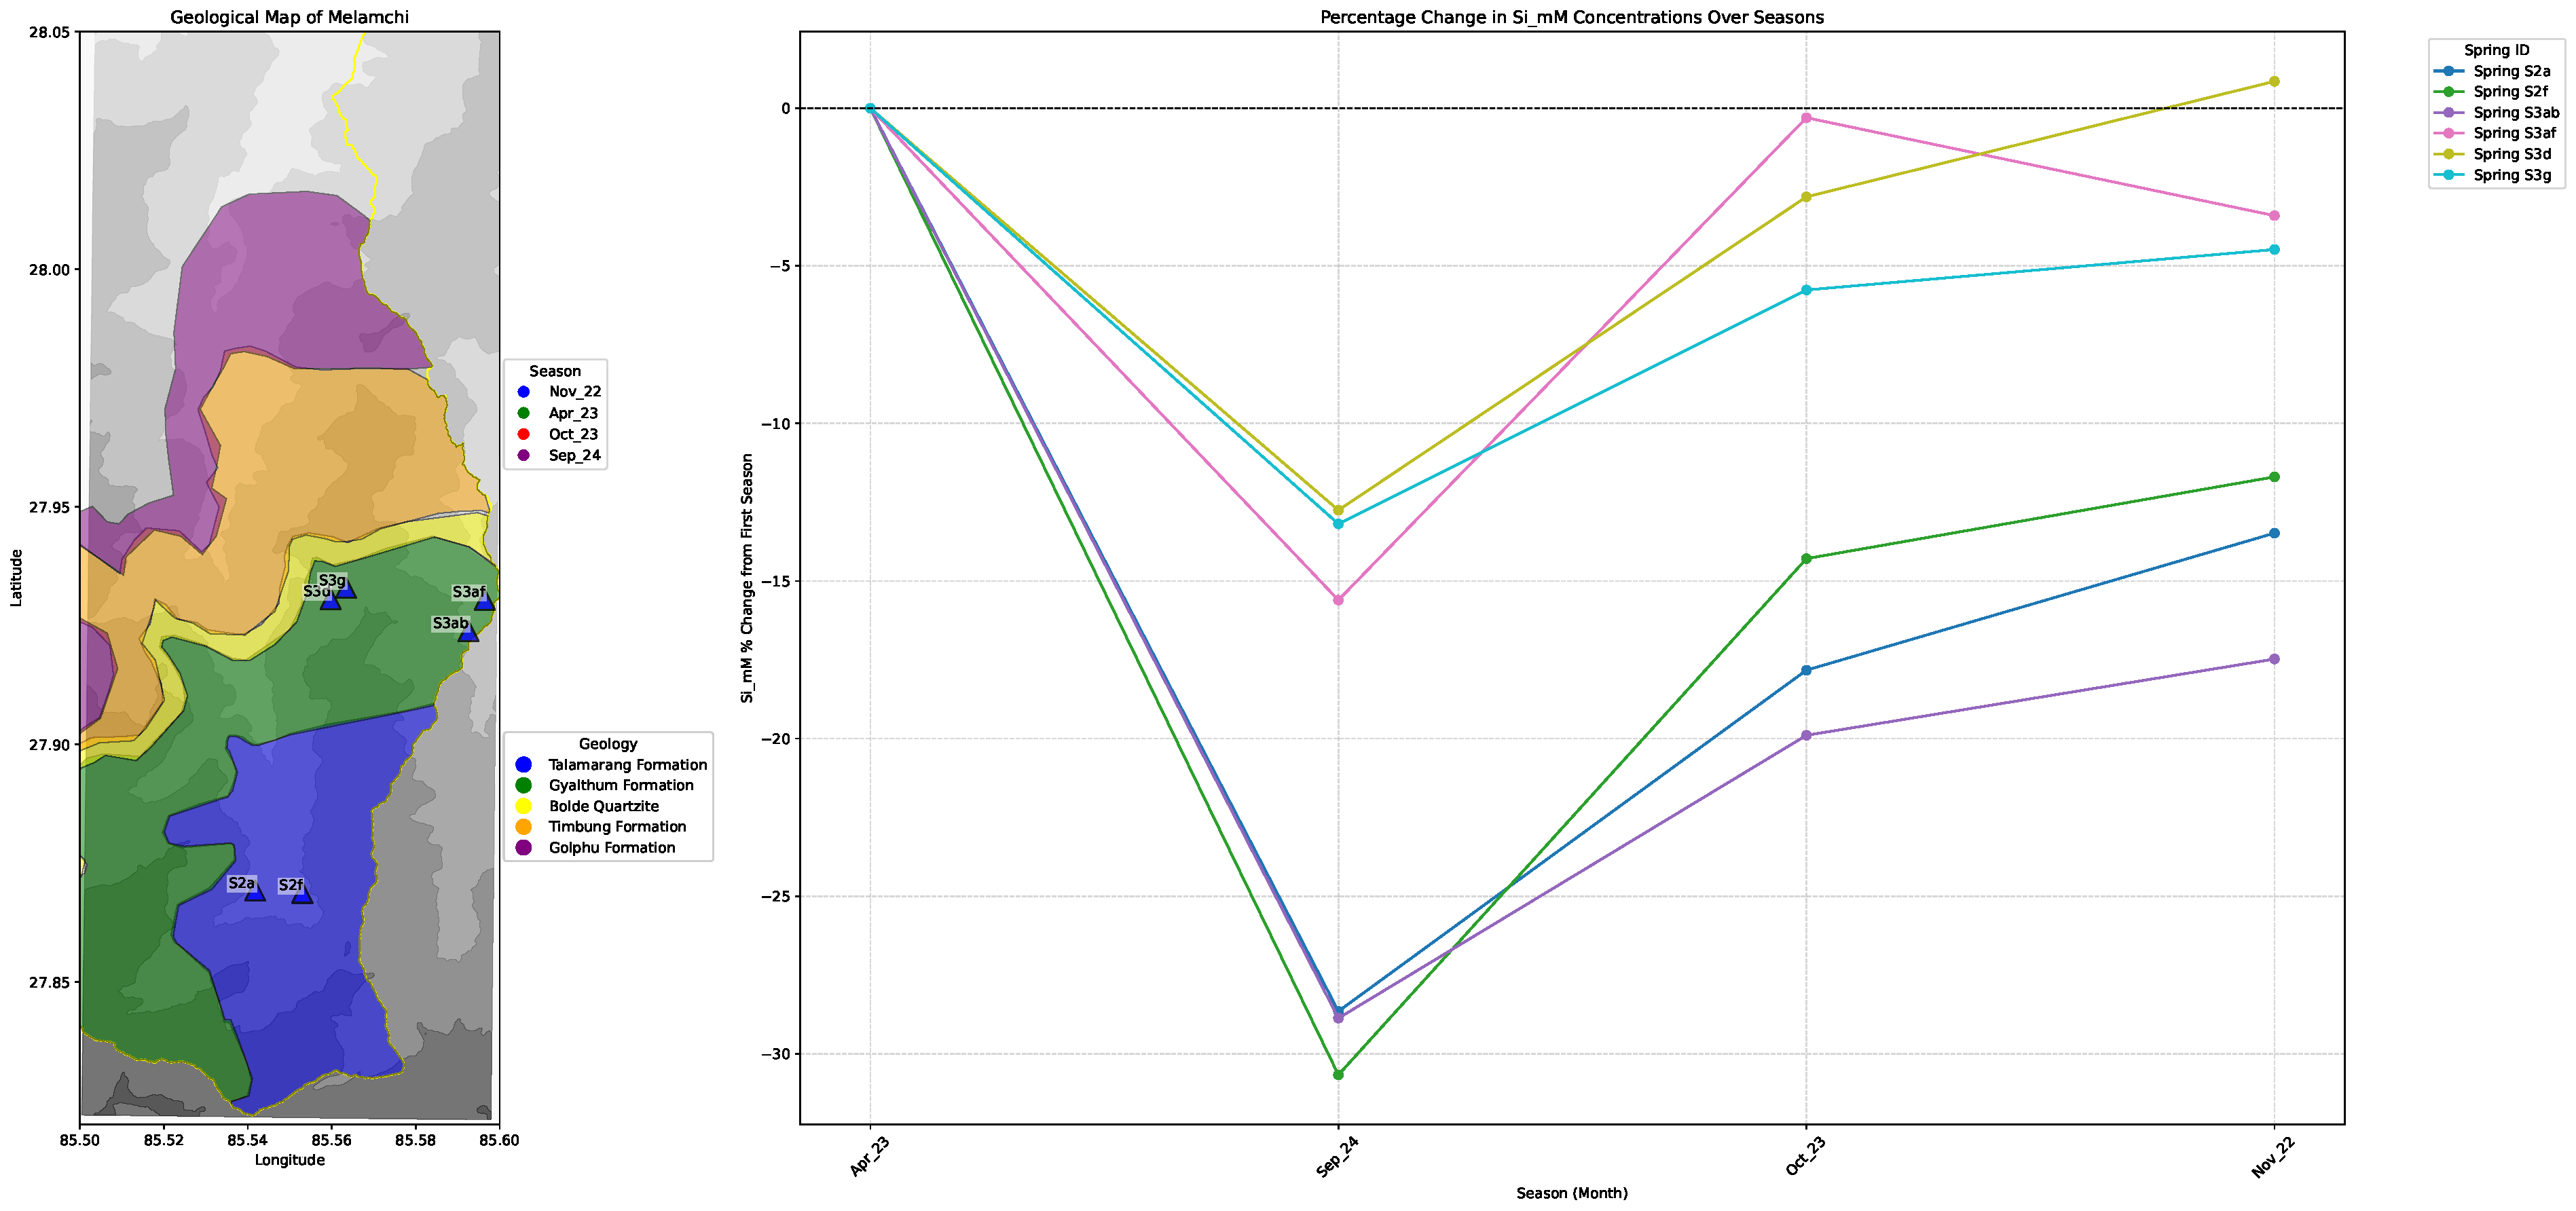
\includegraphics[width=0.8\textwidth]{Si_mM_percentage_change_springs.pdf}
    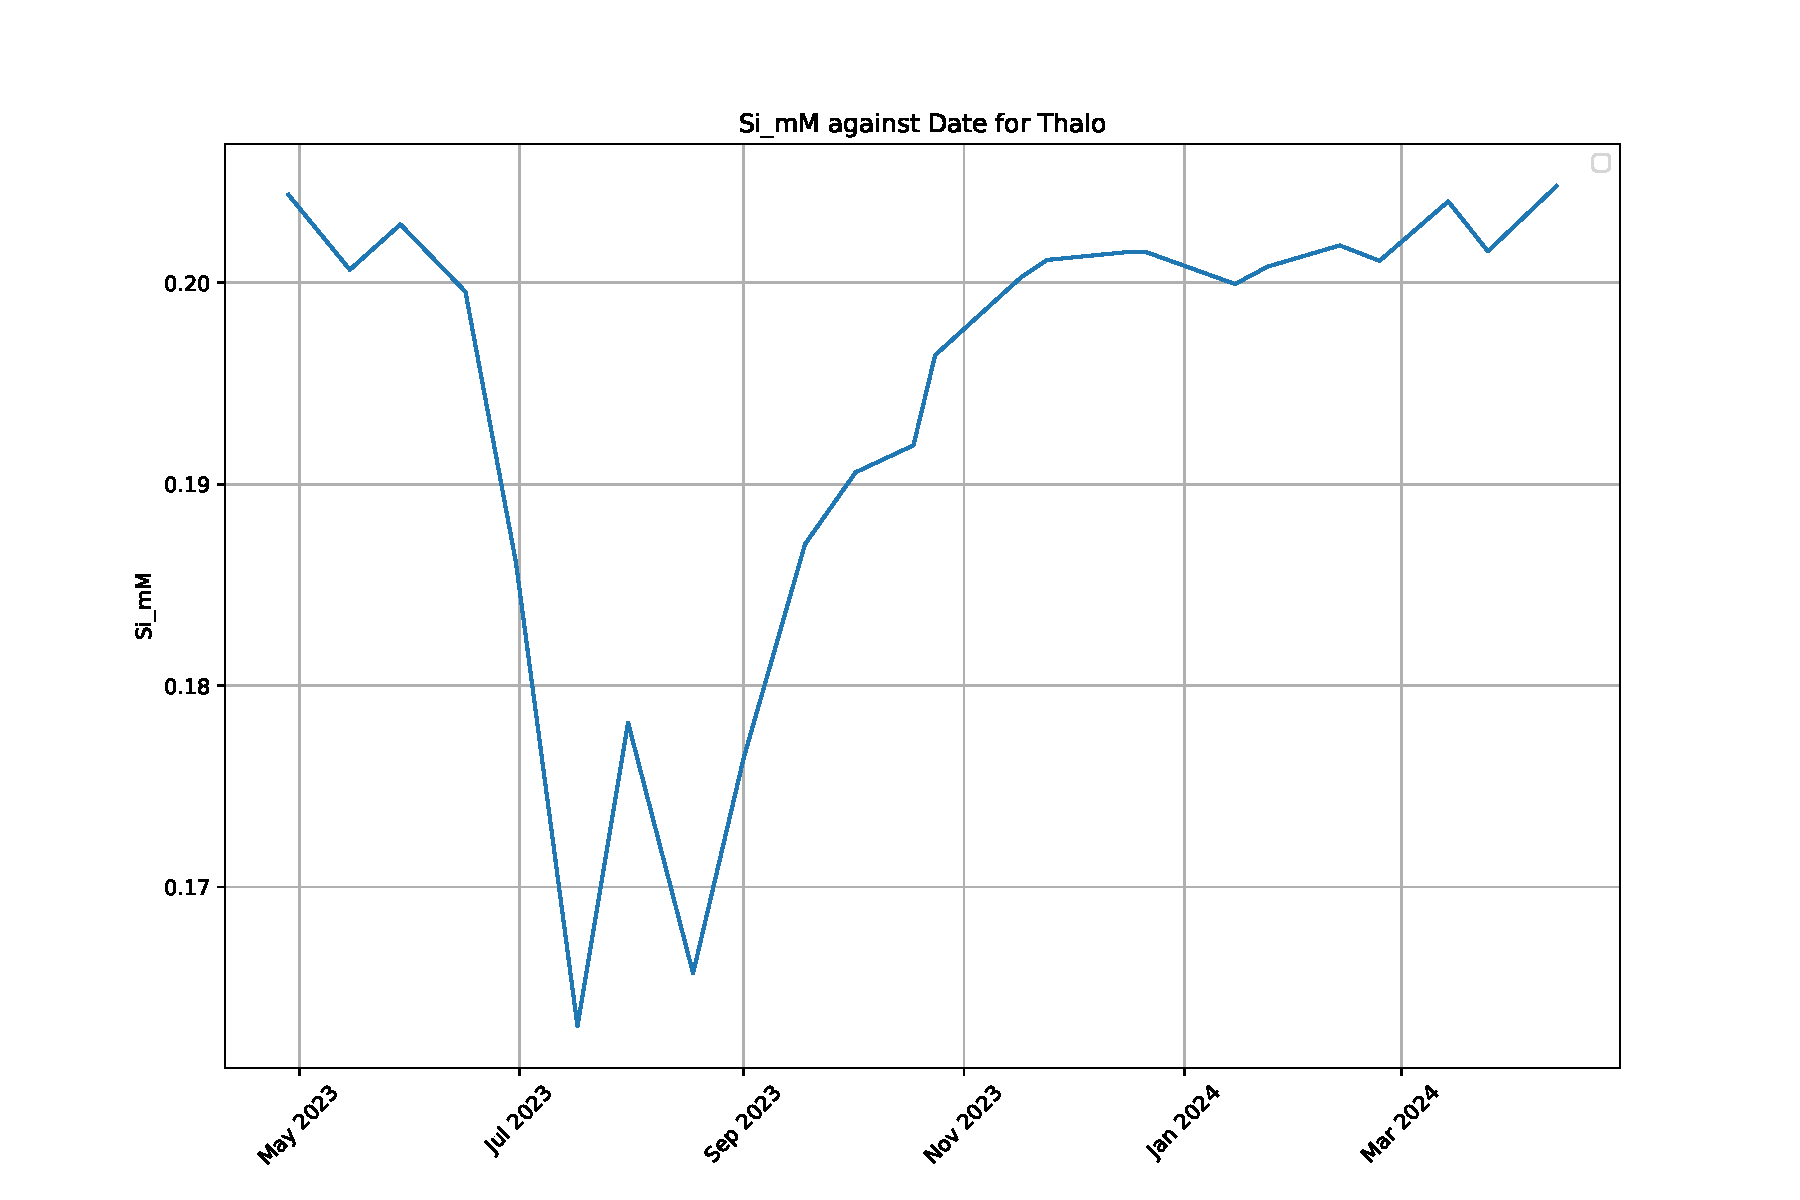
\includegraphics[width=0.8\textwidth]{Si_mM_Thalo_timeseries.pdf}
    \caption{Seasonal changes in spring concentration indicating monsoonal precipitation influence.; Time series of spring concentration changes over time.}
    \label{fig:time_series_changes}
\end{figure}

\FloatBarrier

\bsk

Recorded temperatures at the end of the spring flow paths vary with the season, being coldest in November. All seasons show a temperature decrease with increasing elevation, consistent with the free-air moist adiabatic lapse rate, which is = 6.5 $^{\circ}$C/km (Barry and Chorley, 2009). This differs from the annual mean lapse rate in the southern Himalayas of = 5.2 $^{\circ}$C/km (Kattel et al., 2013). This disparity could be due to the fact that temperatures may be warmer than air temperatures because of radiative heating. The difference may also be due to systematic errors in temperature measurements; between collection and sampling, warming of the water is plausible.



\begin{figure}[h]
    \centering
    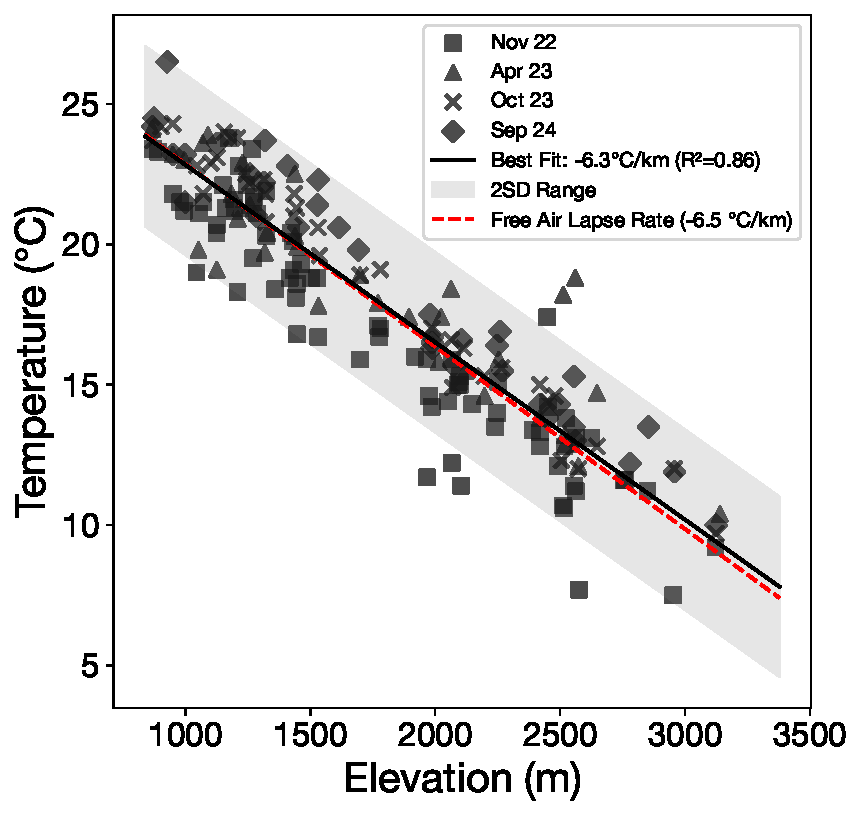
\includegraphics[width=\textwidth]{Temperature_Elevation_Season.pdf}
    \caption{Temperature cahnges}
    \label{fig:seasonal_change2}
\end{figure}

\FloatBarrier

\newpage


\subsection{Spatial Concentration Changes between the Springs}

The northernmost three traverses display a linear trend of concentration with elevation. Alkalinity increases from the north towards the south. This suggests longer flow paths that have had more time to react and accumulate solutes. The southernmost two traverses display a distinct jump in concentration and alkalinity. Southern traverses therefore have a greater deviation from the more dilute rain signature. This could suggest that the springs sampled tap into different lithologies, but this could also be due to longer flow paths and a closer approach to equilibrium. The possible controls on these variations, namely temperature, flow path length, lithology, dissolution rates, and evapotratnspiration cannot easily be distinguished.

\begin{figure}[h]
    \centering
    \begin{tabular}{c}
        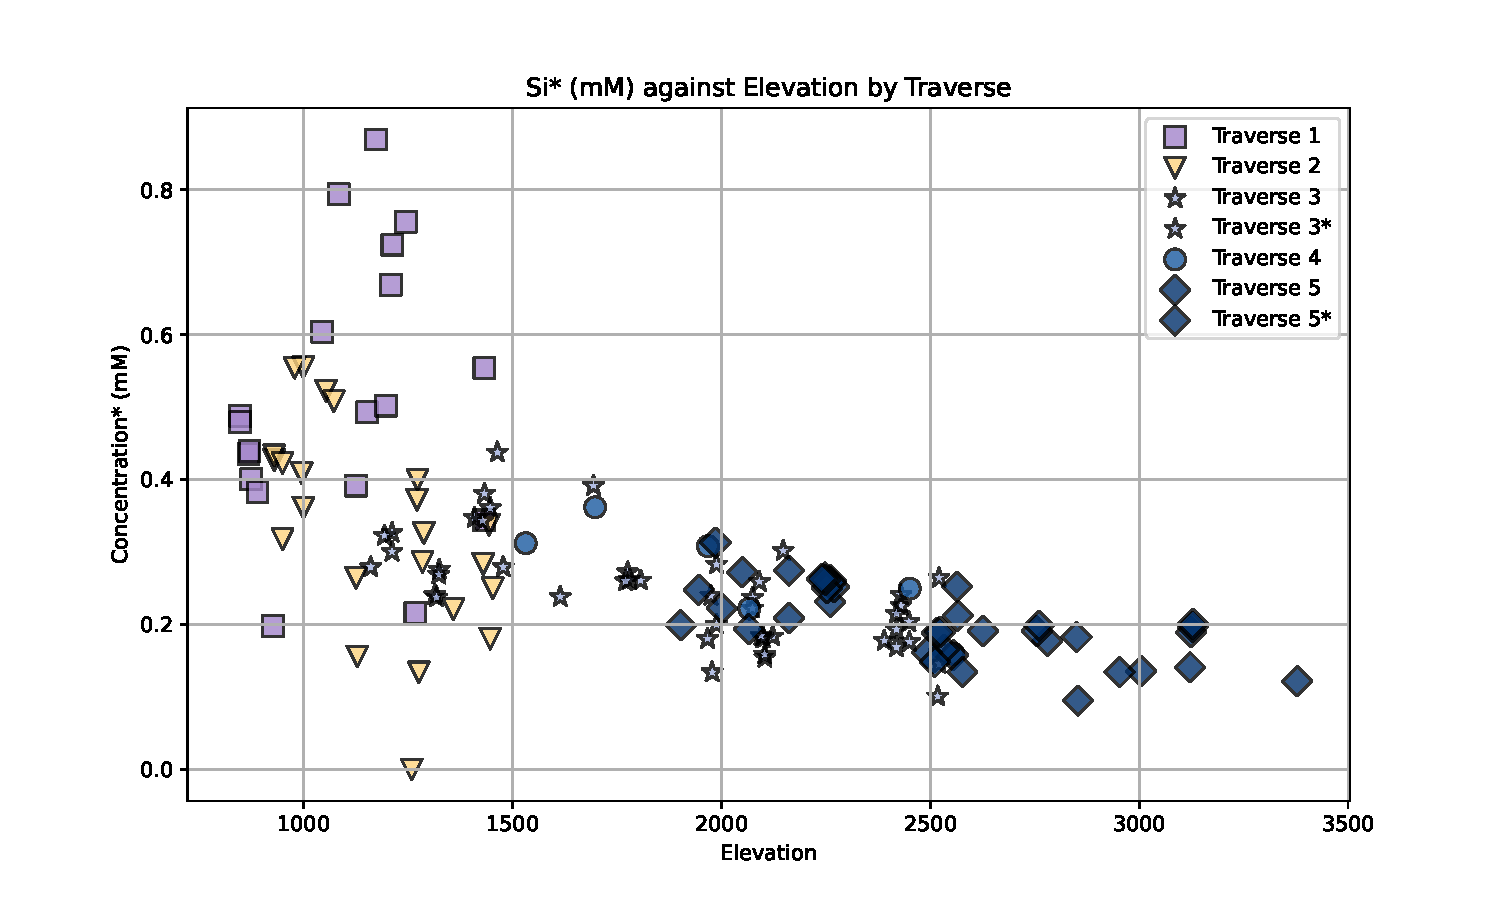
\includegraphics[width=0.8\textwidth]{Si_mM_EC_Elevation.pdf} \\
        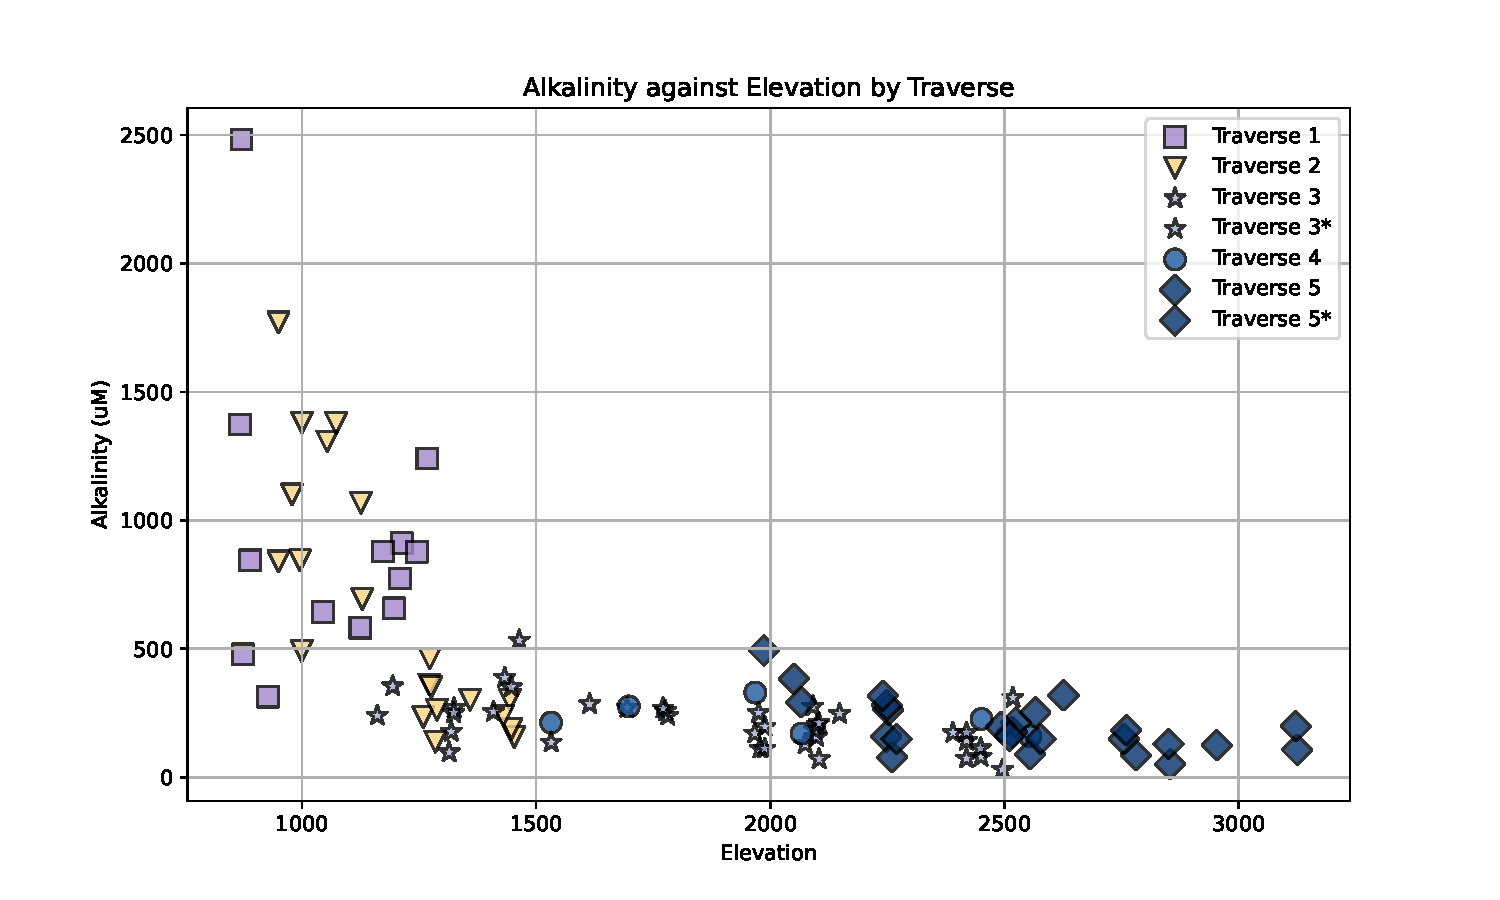
\includegraphics[width=0.8\textwidth]{Alkalinity_Elevation.pdf} \\
    \end{tabular}
    \caption{How Alkalinity and Si changes with elevation}
    \label{fig:spatial_changes_spring2}
\end{figure}

\FloatBarrier

\newpage


\subsection{Strontium isotopes and their Implications}

Radiogenic strontium isotope analyses of springs also show a wide variation between different traverses. Due to the unique source-tracking nature of strontium isotopes this is potentially explained with varying lithology along the ridge. These variations are however consistent with the range of Higher Himalayan Crystalline Series (HHCS) rocks found in the region, so it is unlikely that the source of the Sr isotopes is from the Lesser Himalayan Series (LHS) rocks (Tipper et al., 2006). Indeed the Main Central Thrust (MCT) is several km south of Melamchi.

\bsk

Sr isotopes measured for the collected rain samples range from 0.70904 to 0.73906. Aside from the rain sample collected in the southern Melamchi valley, the Sr isotope values are consistent with the expected values for rainwater (Galy, France-Lenord, Derry, 1999). Furthermore, the lowest Sr isotope value for rain is very close to the reported value for seawater, which is 0.70917. The lowest rain values therefore reflect seawater strontium isotope values, indicating little contamination from dust or particles. The uncontaminated samples are indeed found at the higher elevations, and they show low chloride concentrations consistent with rain.\\

Need to go and look at errors more accurately than this.....\\

\begin{table}[h]
    \centering
    {\footnotesize
    \begin{tabular}{c c c l c l l }
        \hline
        \textbf{Sample ID} & \textbf{Elevation (m)} & \textbf{pH} & \boldmath{$^{87}$Sr/$^{86}$Sr} (\textbf{2SD}$\cdot$10$^{\text{6}}$) & \textbf{Sr ($\mu$M)} & \textbf{Cl ($\mu$M)} & $\delta^{18}$O (\textperthousand) \\
        \hline
        NEP24-039 & 840 & 6.79 & 0.73906 \hfill (24) & 0.13 & 28.09 & -12.23 \\
        NEP24-043 & 1351 & 5.82 & 0.71442 \hfill (46)  & 0.01 & 3.55 & -9.96 \\
        NEP24-044 & 1952 & 6.05 & 0.71352 \hfill (127) & 0.01 & 1.89 & -10.24 \\
        NEP24-045 & 2644 & 5.00 & 0.71292 \hfill (73)  & 0.01 & 3.21 & -11.77 \\
        NEP24-046 & 2110 & 6.02 & 0.70904 \hfill (100) & 0.02 & 2.86 & -10.64 \\
        NEP24-047 & 2644 & 5.74 & 0.71194 \hfill (237) & 0.01 & 0.55 & -15.27 \\
        NEP24-048 & 2644 & 5.61 & 0.71182 \hfill (189) & 0.01 & 3.65 & -15.50 \\
        \hline
        \hline
    \end{tabular}
    }
    \caption{Strontium isotope ratios, chloride and strontium concentrations (in micromolar, \textmu M), elevation, pH, and $\delta^{18}$O values (‰ VSMOW). Error (2SD) values are multiplied by $10^6$.}
    \label{tab:sr87_sr86_data}
\end{table}



Strontium isotope ratios used alongside strontium concentrations can be used to determine mixing between different endmembers (Faure, 1986; See Appendix). Plots of $\ddfrac{^{87}Sr}{^{86}Sr}$ against $\ddfrac{1}{Sr}$ that yield straight lines are indicative of mixing trends. 

\begin{figure}[p]
    \centering
    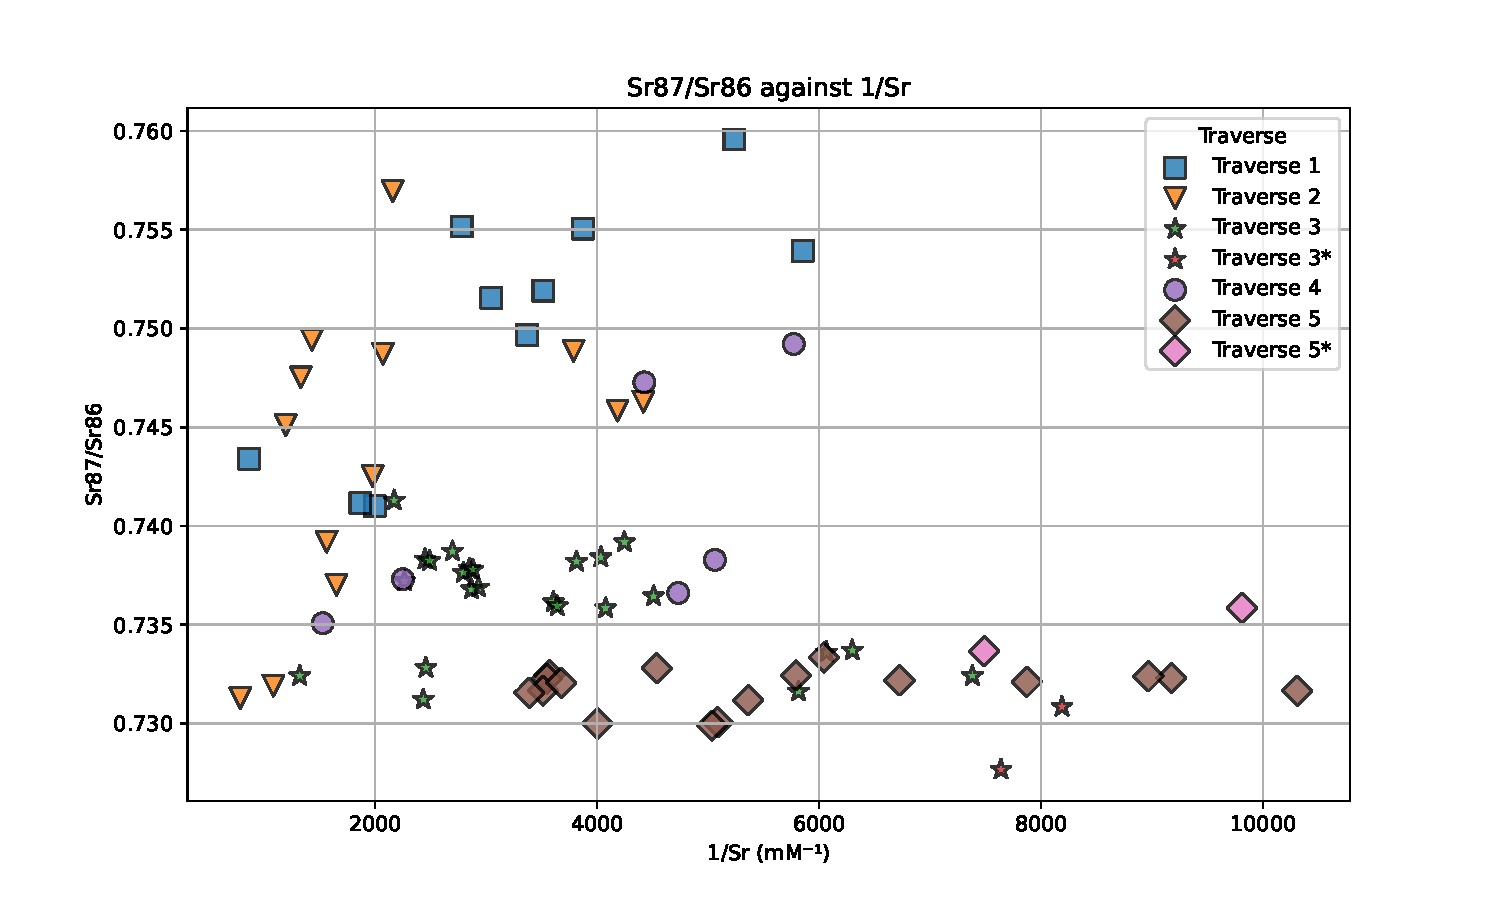
\includegraphics[width=\textwidth]{Sr87_Sr86_1_Sr.pdf}
    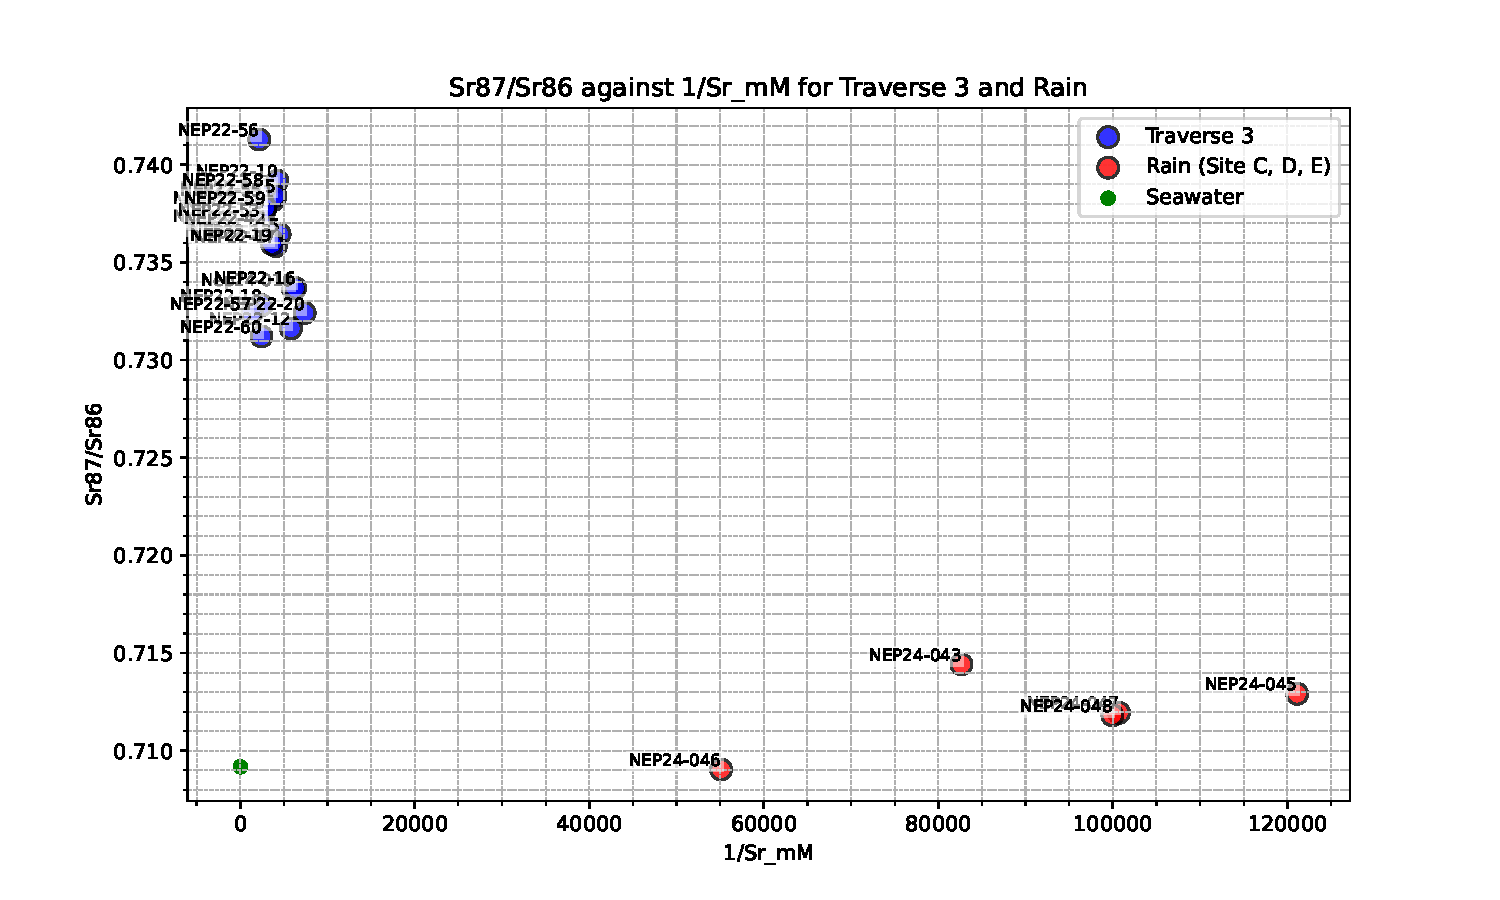
\includegraphics[width=\textwidth]{Sr87_Sr86_1Sr_Rain.pdf}
    \caption{Strontium isotope differences display difference in lithology tapped in. Cite Quade and Tipper papers; Rain analysed for Sr isotopes and Cl. Something about contamination lower down; How samples of Traverse 3 compare to the rain samples}
    \label{fig:discussion3}
\end{figure}

\FloatBarrier

Figure \ref{fig:discussion3}a shows $\ddfrac{^{87}Sr}{^{86}Sr}$ against $\ddfrac{1}{Sr}$ for springs in the catchment. The plot shows two distinct mixing lines between Traverses 1-3, and Traverses 3-5 [need to draw them on]. This supports that found in figure \ref{fig:spatial_changes_spring2}, which suggests the water chemistry in Traverses 1 and 2 is quite different to the trend set by Traverses 3-5. Comparing spring samples to the rain [Change graph], it is clear that the latter does not exert a significant control on the spring chemistry, not even for the presumably shortest flow paths at the top of the ridge. In other words, chemical weathering reactions are likely to be the main control on the spring chemistry.


\newpage

\subsection{Consistent Flow Paths Mid-Catchment}

It is difficult to explain the inter-traverse variation in concentration and isotopic composition. As a result, for the remainder of this study's analysis, only Traverse 3 out of the five will be chosen as a case study representing the catchment. It is possible, and quite likely given the aforementioned mixing trends that all traverses' flow paths are connected one to the other. However, focusing on one traverse allows the contribution of spatial variation toward the overall chemistry to be minimised. 

\bsk

For Traverse 3, there is evidence to suggest lithology is largely constant. For one, geological maps suggest lithology does not vary across E-W, which is the profile all traverses follow. Secondly, the narrow range and tight scatter in Figure \ref{fig:spatial_changes_spring8} for Na/Si suggests little lithological change and consistently sampled flow paths over time. Na/Si plots almost exactly on the 1:1 line for every season where the same spring was sampled in Traverse 3. The fact that this ratio increases with decreasing elevation makes sense given Si is involved in the backward secondary mineral precipitation weathering reaction, and Na is not. In other words, elevated Na/Si is interpreted as a sign of a closer approach to equilibrium, as more Si is scavenged from the water to form secondary precipitates, while the Na is only involved in dissolution. This is even more apparent when plotting against elevation. 

\begin{figure}[h]
    \centering
    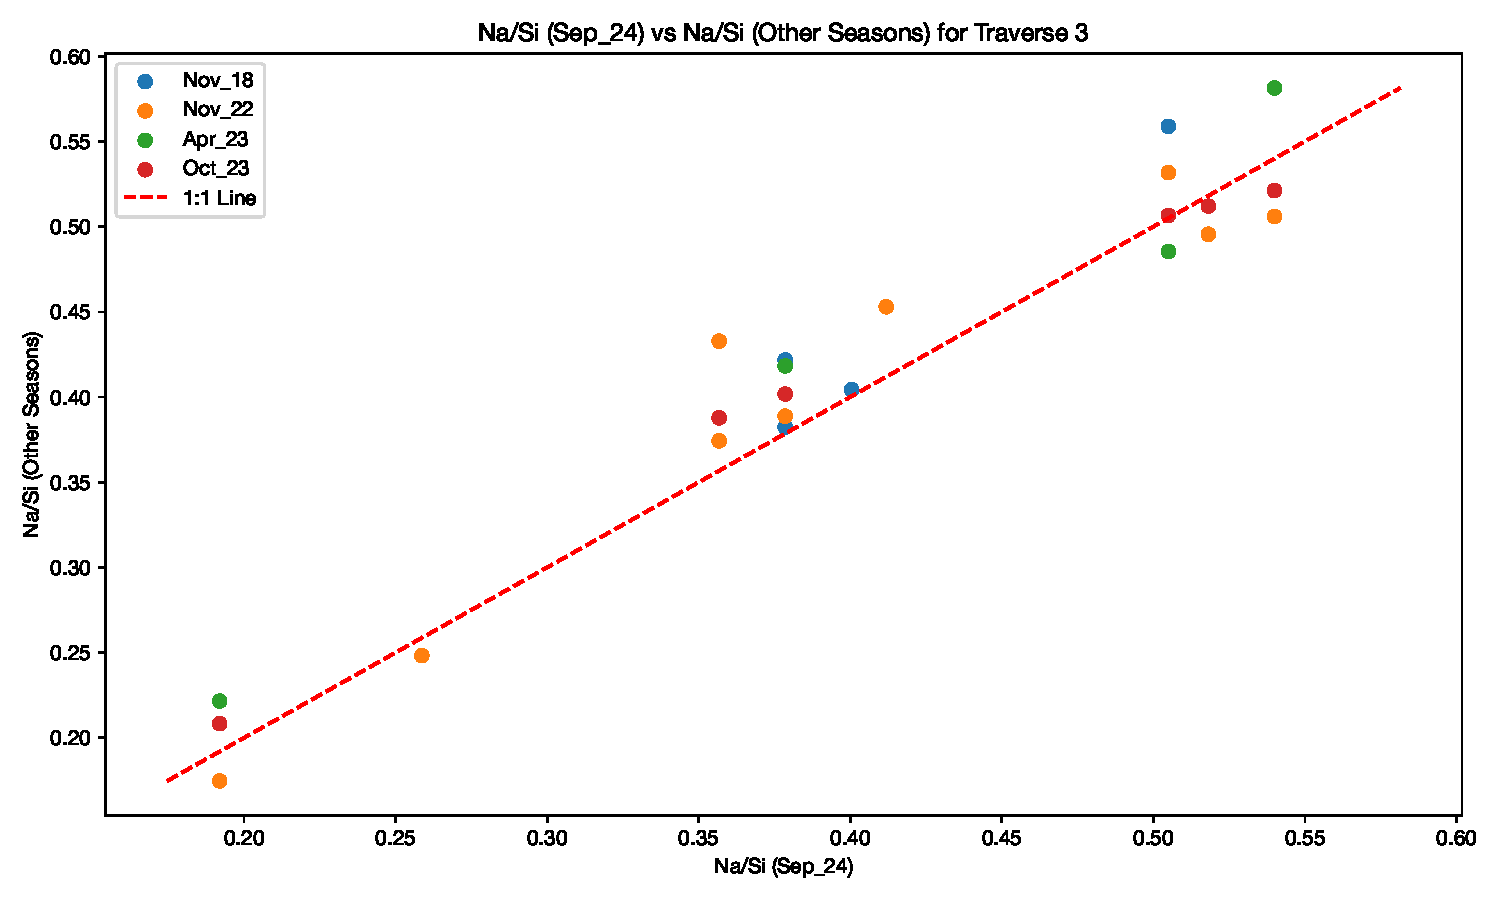
\includegraphics[width=\textwidth]{Na_Si_Trav3.pdf}
    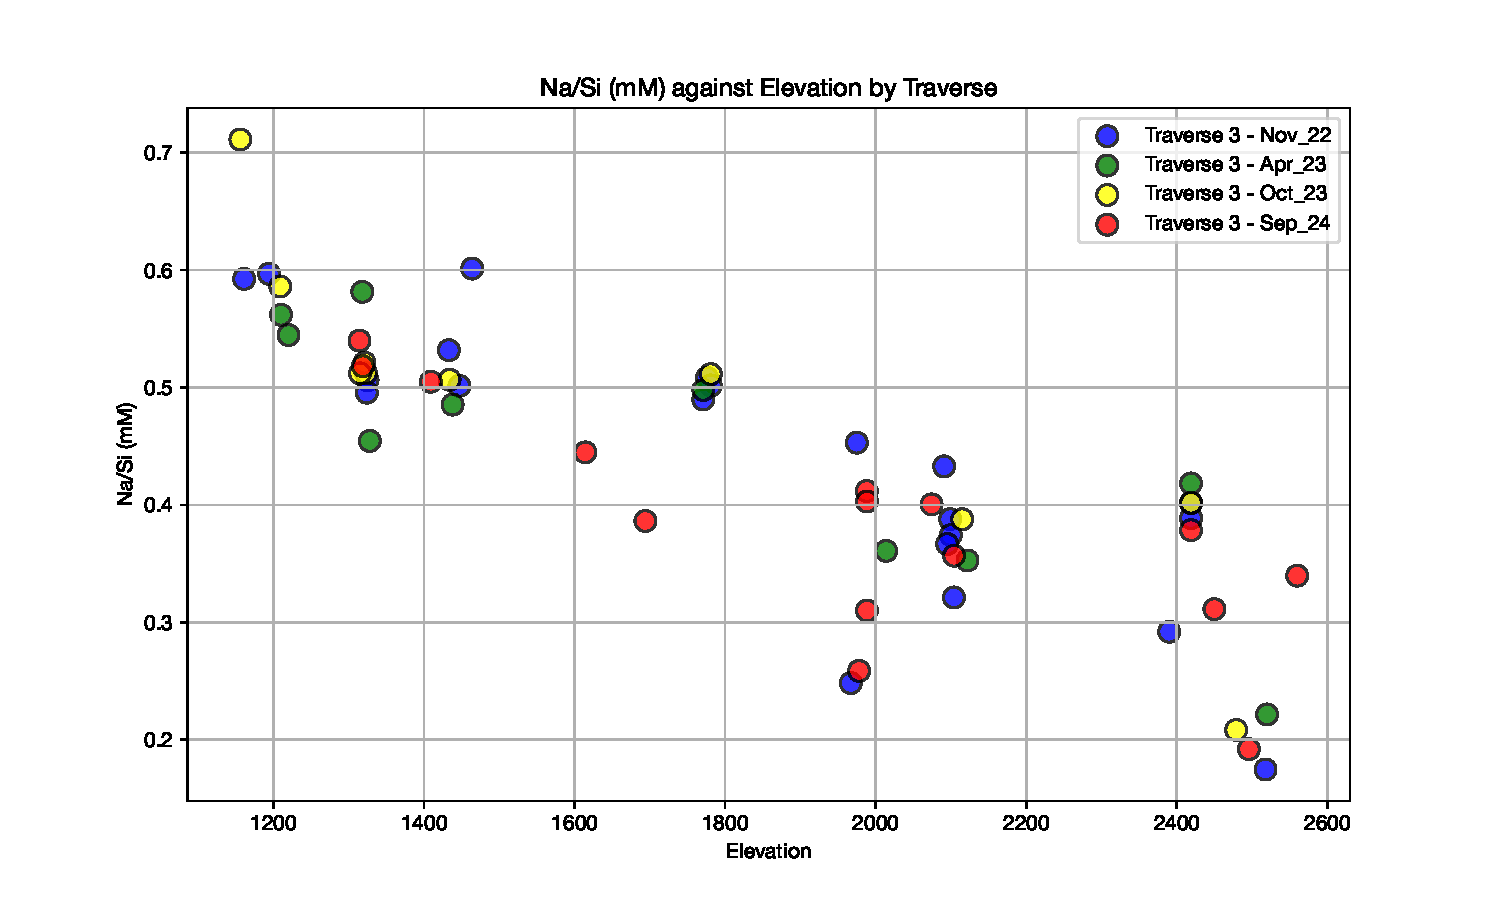
\includegraphics[width=\textwidth]{Na_Si_Elevation.pdf}
    \caption{How Si varies for Traverse 3, showing a wide variety of samples; Na/Si for Traverse 3 is pretty neat. Consistently sampled flow paths.}
    \label{fig:spatial_changes_spring8}
\end{figure}
\FloatBarrier

Figure \ref{fig:spatial_changes_spring9} shows the Na/Si ratio for the springs sampled over a time series. The Thalo spring exits in Traverse 3. The three springs displayed in Figure  \ref{fig:spatial_changes_spring9} largely follow the same spatial Na/Si trend as that shown in \ref{fig:spatial_changes_spring8} (plot needed to show the spatial extent in Figure \ref{fig:spatial_changes_spring8}). An outlier, however, is the spike in Na/Si shortly after the start of the monsoon, suggesting temporal variation in flow paths. There is an argument to be made for this to be a spurious measurement due to its very large deviation from the other samples in the Thalo timeseries. The spike is not just formed by one point, though. Around it the sampled points form a trough of sorts, suggesting that there is an approach to a high Na/Si signature. This spike is interpreted as the mobilisation of more concentrated, older water in the subsurface due to an increased water flux. In other words, the increased precipitation from the monsoon leads to flowpaths that sample deeper, older water that is closer to equilibrium.

 \begin{figure}[h]
    \centering
    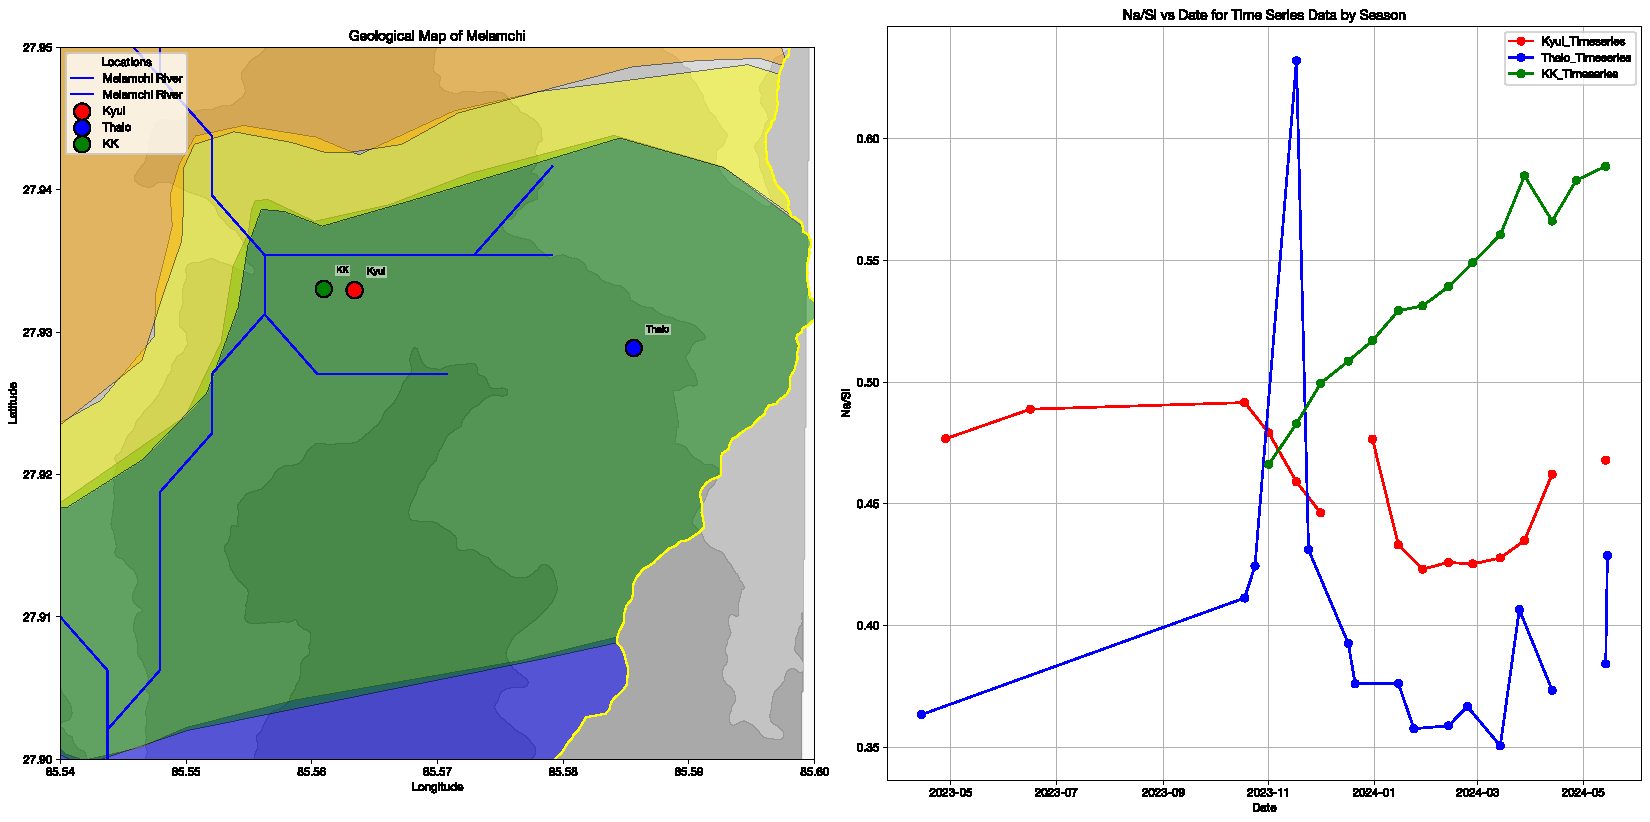
\includegraphics[width=\textwidth]{Na_Si_thalo.pdf}
    \caption{Na/Si for Thalo Timeseries}
    \label{fig:spatial_changes_spring9}
\end{figure}
\FloatBarrier

Traverse 3 therefore has consistent flow paths, scope for reactive transport modeling, and displays temporal variation in response to monsoonal precipitation. This makes it the optimal traverse for modeling the catchment.


